\documentclass{article}
\usepackage[utf8]{inputenc}
\usepackage{graphicx} % Required for \includegraphics
\usepackage{amsmath} % For mathematical typesetting
\usepackage{hyperref} % For clickable links in references
\usepackage{booktabs} % For better table rules
\usepackage{geometry} % To adjust page margins
\usepackage{setspace} % For custom line spacing
\usepackage{mathptmx} % For Times New Roman-like font
\geometry{a4paper, margin=1in} % Set A4 paper with 1-inch margins

\title{Faster Korean BERT Fine-tuning with Sequence Length Bucketing}
\author{Beomyong Choi}
\date{September 23, 2025} % Today's date

\begin{document}
\setstretch{1.1}

\maketitle

\begin{abstract}
Fine-tuning allows a pre-trained model to adapt to a specific task by training it further on data closely related to the task domain. Compared to building a model entirely from scratch, this process is much faster and less computationally demanding. (Devlin et al., 2018)

However, a  substantial segment of the remaining inefficiency comes from the padding needed when dealing with batches of text that vary in length. To address this without altering the underlying model architecture, our work focuses on improving the data pipeline itself.

In particular, we explore the use of bucketing, a technique that groups samples of similar length to minimize padding waste. When applied to \texttt{klue/bert-base} on the Korean NSMC dataset, bucketing removed nearly all padding tokens—99.99\% in total. This change produced a 3.6$\times$ increase in training speed, reducing total time by 73\%, while maintaining almost identical accuracy (90.51\% vs. 90.47\%).

These findings show how even small changes can make LLM fine-tuning more efficient and practical.
\end{abstract}

\section{Introduction}

The pre-train and fine-tune paradigm, introduced by models like BERT (Devlin et al., 2018), is now foundational to modern NLP. This approach allows large models to be adapted for specific tasks with minimal additional training, achieving state-of-the-art performance without the prohibitive cost of training from scratch. In Korean NLP, models such as KLUE-BERT (Park et al., 2021) exemplify this success. However, despite this efficiency, fine-tuning large models remains a substantial hurdle because of the high demand for computational resources and time, which hinders rapid experimentation.

This inefficiency is driven in large part by the padding required for batch processing. To take advantage of GPU parallelization, all sequences in a batch must have a uniform length. This requirement necessitates adding \texttt{[PAD]} tokens to shorter sequences, and although semantically meaningless, these tokens are included in computations. The result is wasteful overhead that inflates the total training time.

Although much research has focused on architectural changes to improve efficiency, our work concentrates on the data processing pipeline. We apply and analyze the effects of bucketing, a well-known technique that groups similarly-sized data to reduce padding. Our experiments on the NSMC dataset demonstrate that bucketing can dramatically improve the training speed of KLUE-BERT without sacrificing model performance.

\section{Background}

This section outlines the key technical concepts for our study. We describe the model and dataset used, followed by an explanation of padding inefficiency and the bucketing technique.

\subsection{Language Model: KLUE-BERT}
We used the \texttt{klue/bert-base} model (Park et al., 2021) for our experiments. KLUE-BERT is a language model based on the Transformer architecture (Vaswani et al., 2017). It was pre-trained on a large Korean corpus for various NLP tasks.

\subsection{Benchmark Dataset: NSMC}
The Naver Sentiment Movie Corpus (NSMC) serves as our benchmark dataset. It contains 200,000 movie reviews labeled with positive (1) or negative (0) sentiment and includes standard training and test splits.

\subsection{The Challenge: Padding Inefficiency}
A key challenge in training with text data is the inefficiency caused by padding. To leverage GPU parallelization, deep learning models process data in batches of uniform-sized tensors. Since sentences have varying lengths, shorter sequences must be padded with special \texttt{[PAD]} tokens to match the longest sequence in a batch. These tokens, while semantically meaningless, are included in GPU computations and lead to wasted resources and longer training times.

\subsection{The Solution: Bucketing}
Bucketing is a data sampling technique used to address padding inefficiency. The method works by sorting the dataset by sequence length before training. Batches are then formed by grouping sequences of similar lengths, which minimizes the amount of required padding and improves training efficiency.

\section{Methodology}

This section details our experimental design for testing bucketing efficiency. We describe the baseline training approach, our bucketing implementation, and the evaluation metrics used.

\subsection{Baseline Model: Static Padding}
Our baseline follows standard BERT fine-tuning with static padding. In this method, all NSMC sentences were tokenized using the \texttt{klue/bert-base} tokenizer and then padded or truncated to a fixed \texttt{max\textunderscore length} of 128. We used the HuggingFace \texttt{Trainer} API with standard settings for fine-tuning: 3 training epochs, a batch size of 32, a learning rate of 5e-5, and a weight decay of 0.01. Evaluation occurred every 1000 steps. The model was fine-tuned on the complete NSMC training set, and the resulting training time and final accuracy serve as our comparison baseline.

\subsection{Proposed Method: Dynamic Padding with Bucketing}
Our proposed method uses an identical architecture and the same hyperparameters as the baseline but optimizes the data pipeline. We first tokenized and truncated sentences without applying padding. Then, we enabled two key \texttt{Trainer} configurations for efficiency: we used a \texttt{DataCollatorWithPadding} to dynamically pad each batch to its longest sequence, and enabled the \texttt{group\textunderscore by\textunderscore length=True} argument, which causes the \texttt{DataLoader} to group similar-length sequences into batches. This combination reduces padding tokens per batch and cuts wasted computation.

\subsection{Evaluation Metrics}
We assess our method on two dimensions: performance and efficiency. Model performance is measured by \textbf{Accuracy}—the percentage of correct classifications on the test set. Training efficiency is measured by \textbf{Total Training Time}—the wall-clock time from the start to completion of the \texttt{trainer.train()} function.

\subsection{Experimental Setup}
All experiments were conducted in a Google Colab environment, equipped with a single NVIDIA Tesla T4 GPU, using PyTorch and the Hugging Face Transformers (v4.56.1) library.

\section{Results}

We compared the baseline (static padding) and bucketing methods on both efficiency and performance. The results in Table \ref{tab:performance} and Figure \ref{fig:comparison} show training speed improvements with minimal accuracy loss.

\begin{table}[htbp]
\centering
\caption{Performance and Efficiency Comparison}
\label{tab:performance}
\begin{tabular}{llll}
\toprule
No. & Methodology & Training Time (min) & Final Accuracy (\%) \\
\midrule
1 & Baseline (Static Padding) & 236.37 min & 90.51 \% \\
2 & \textbf{Proposed (Bucketing)} & \textbf{64.63 min} & \textbf{90.47 \%} \\
\bottomrule
\end{tabular}
\end{table}

\begin{figure}[htbp]
\centering
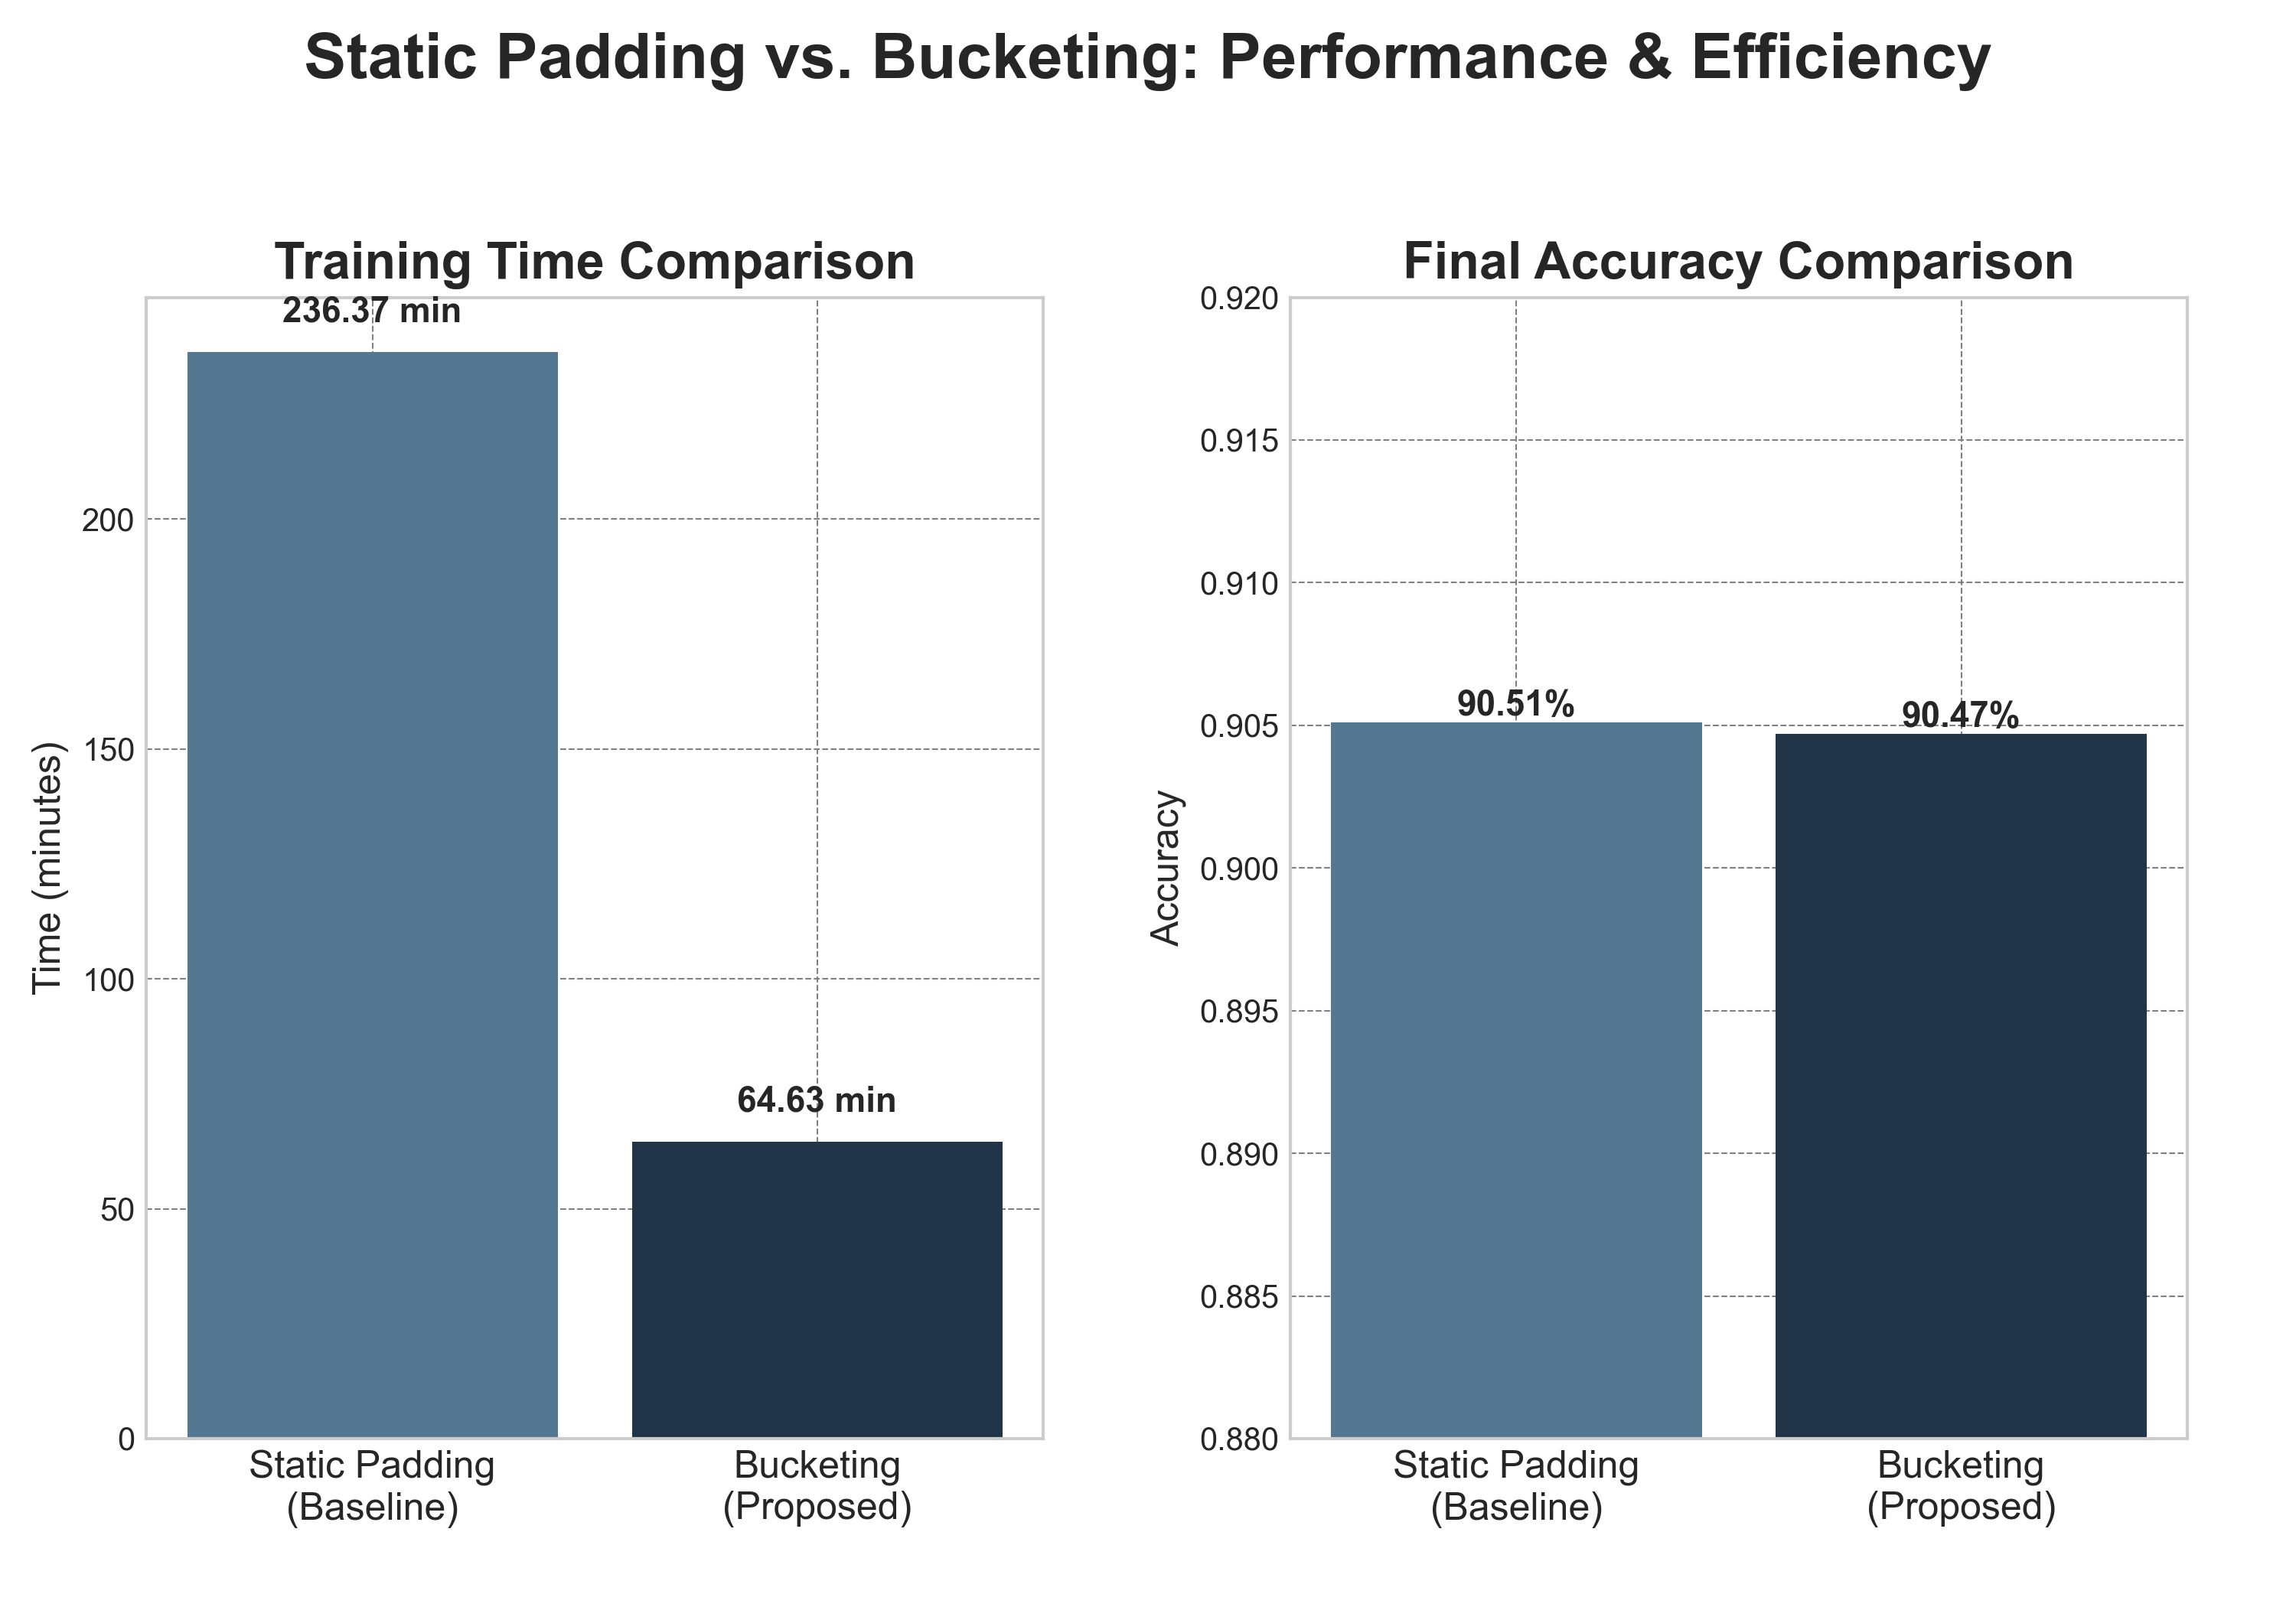
\includegraphics[width=0.8\textwidth]{comparison_graph_eng_v3.png}
\caption{Comparison of Training Time and Accuracy}
\label{fig:comparison}
\end{figure}

\subsection{Training Efficiency}
The most notable finding is a 3.6$\times$ speedup in training time. The baseline model took approximately 236 minutes to complete, while the bucketing method finished in just 65 minutes. This efficiency gain stems from the sharp reduction in processed \texttt{[PAD]} tokens. Static padding processed 15,858,683 padding tokens, while our method processed only 1,851—representing a 99.99\% reduction.

\subsection{Model Performance}
This improvement in training speed came with virtually no performance cost. The bucketing method achieved 90.47\% accuracy, differing by only 0.04 percentage points from the baseline's 90.51\%. This confirms that our optimization improves efficiency while maintaining the model's predictive capability.

\section{Conclusion}

We set out to test whether bucketing could make Korean language model fine-tuning more practical. The results were clearer than expected: a 3.6$\times$ speedup with essentially no accuracy cost.

The mechanism is simple: by grouping similar-length sequences to minimize padding waste, our method eliminated 99.99\% of padding tokens on the NSMC dataset and cut training time by 73\%. The resulting accuracy difference of just 0.04 percentage points falls well within normal variation.

While these gains are most pronounced on variable-length datasets common in real-world NLP, other efficiency techniques would be more appropriate for domains with uniform-length text.

For practitioners, this represents an easy win. The implementation requires minimal code changes but delivers substantial time savings—valuable for any team doing frequent model experimentation.

\section{References}
\begin{thebibliography}{99}

\bibitem{devlin2018bert}
Devlin, J., Chang, M. W., Lee, K., \& Toutanova, K. (2018). \textit{Bert: Pre-training of deep bidirectional transformers for language understanding}. arXiv preprint arXiv:1810.04805.

\bibitem{park2021klue}
Park, W., Lee, J., Kim, S., Kim, M., Kim, D., \& Cho, K. (2021). \textit{KLUE: Korean Language Understanding Evaluation}. arXiv preprint arXiv:2105.09680.

\bibitem{vaswani2017attention}
Vaswani, A., Shazeer, N., Parmar, N., Uszkoreit, J., Jones, L., Gomez, A. N., ... \& Polosukhin, I. (2017). \textit{Attention is all you need}. In Advances in neural information processing systems (pp. 5998-6008).

\bibitem{huggingface2024transformers}
Hugging Face. (2024). \textit{Transformers Documentation}. \url{https://huggingface.co/docs/transformers}

\end{thebibliography}

\end{document}